\documentclass[12pt, a4paper]{report}

\usepackage{geometry}
\geometry{a4paper, left=30mm, right=20mm, top=30mm, bottom=30mm}

\usepackage{hyperref}
\usepackage{t1enc}
\usepackage[utf8]{inputenc}
\usepackage[magyar]{babel}
\usepackage{amsmath}
\usepackage{amsfonts}
\usepackage{algorithm}
\usepackage{algpseudocode}
\usepackage{amsthm}
\usepackage{listings}
\usepackage{color}
\usepackage{xcolor}
\usepackage{colortbl}
\usepackage{caption}
\usepackage{subcaption}
\usepackage{ellipsis}
\usepackage{multirow}
\usepackage{tocloft}

\usepackage[autostyle]{csquotes}
\selectlanguage{magyar}
\DeclareQuoteAlias{dutch}{magyar}

\usepackage{apacite}
\bibliographystyle{apacite}

\usepackage{url}
\usepackage{textcomp}

\usepackage{tikz}
\usetikzlibrary{shapes}
\usetikzlibrary{positioning}

\usepackage[decimalsymbol=comma]{siunitx}

\usepackage[linewidth=0.33pt, rightline=false, leftline=false, framemethod=tikz]{mdframed}

\usepackage{graphicx}
\graphicspath{ {./images/} }

% Különleges karakterek használatának lehetősége kódrészletben
\lstset{literate=
 {á}{{\'a}}1 {é}{{\'e}}1 {í}{{\'i}}1 {ó}{{\'o}}1 {ú}{{\'u}}1
 {Á}{{\'A}}1 {É}{{\'E}}1 {Í}{{\'I}}1 {Ó}{{\'O}}1 {Ú}{{\'U}}1
 {ö}{{\"o}}1 {ü}{{\"u}}1 {Ö}{{\"O}}1 {Ü}{{\"U}}1
 {ű}{{\H{u}}}1 {Ű}{{\H{U}}}1 {ő}{{\H{o}}}1 {Ő}{{\H{O}}}1
}

\definecolor{codegray}{rgb}{0.5,0.5,0.5}
\lstset{xleftmargin=15pt,
        basicstyle=\scriptsize,
        numbers=left,
        numbersep=5pt,
        numberstyle=\tiny\color{codegray},
        escapechar=@,
        aboveskip=2em,
        belowskip=2em,
        belowcaptionskip=2em}

\renewcommand{\lstlistingname}{Kódrészlet}

\renewcommand\BOthers{és mtsai\hbox{}}
\renewcommand\BOthersPeriod{és mtsai.\hbox{}}
\renewcommand\BRetrievedFrom{Letöltve:\ }
\renewcommand\BRetrieved[1]{Letöltve, {#1}:\ }
\renewcommand\BIn{}
\renewcommand\BED{Szerk. \hbox{}}
\renewcommand\BEDS{Szerk. \hbox{}}
\renewcommand\BMTh{Diplomamunka}
\renewcommand{\BCBT}{}
\renewcommand{\BCBL}{}

\renewcommand{\ellipsisgap}{0.1em}

\linespread{1.25}

\providecommand{\useColors}{1}

\newtheorem*{definition*}{Definíció}

\providecommand*{\printsecond}[2]{#2}

\renewcommand\cftchapafterpnum{\vskip2pt}

\newcommand{\dotref}[1] {\ref{#1}.}

\newenvironment{outdentlist}
  {\begin{list}{}{\setlength\itemindent{-\leftmargin}}}
  {\end{list}}

\theoremstyle{definition}
\newtheorem{definition}{Definíció}


\begin{document}
    % University Assignment Title Page 
% LaTeX Template
% Version 1.0 (27/12/12)
%
% This template has been downloaded from:
% http://www.LaTeXTemplates.com
%
% Original author:
% WikiBooks (http://en.wikibooks.org/wiki/LaTeX/Title_Creation)
%
% License:
% CC BY-NC-SA 3.0 (http://creativecommons.org/licenses/by-nc-sa/3.0/)

\begin{titlepage}

\center

{\huge \bfseries {{Nulla-ismeretű protokollok}}}\\[1.5cm]

\textsc{\Large {{Vécsi Ádám}}}\\
\textsc{\large {{Debreceni Egyetem Informatikai Kar}}}\\
\textsc{\large {{Számítógéptudományi Tanszék}}}

\vfill

\end{titlepage}


    \setlength{\cftbeforechapskip}{.2ex}
    \setlength{\cftbeforesecskip}{-.5ex}
    \tableofcontents

    \chapter{Bevezetés}

Az entitások/felhasználók autorizácijó az internet terjedésével egyre gyakoribb folyamattá válik. A legelterjedtebb és legkézenfekvőbb módja ennek a jelszavak használata. A felhasználó a regisztráció során megad egy karaktersorozatot, amelyet a szerver eltárol, így belépéskor csupán össze kell hasonlítanunk, hogy a kapott jelszó megegyezik-e a tárolttal. Nem igényel bonyolult matematikai folyamatokat, letisztult folyamat. Azonban ez a módszer számos hátulütővel rendelkezik. Kezdjük azzal, hogy a http protokoll nem kínál titkosított kommunikációs csatornát, így egy közbeékelődéses (man-in-the-middle) támadással könnyedén kompromitálódhat jelszavunk és jelentős károkat szenvedhetünk. A https megjelenésével azonban a TLS/SSL rétegnek köszönhetően biztonságos, titkosított csatornákhoz juthatunk ezzel hátráltatva/megakadályozva a titkos adataink kompromitációját.

Ez azonban nem nyújt számunkra teljes védelmet, hiszem a támadások célpontjai közt szerepelnek a szerverek, amiken a jelszavaink tárolásra kerültek. Mivel egyre több szolgáltatás jelenik meg, újabb és újabb felhasználói fiókokat regisztrálunk és az esetek többségében a jelszavunk megegyezik. Ha bármelyik szolgáltatás ellen sikeres támadást halytanak végre, akkor ennek akár több felhasználói fiókunk is kárát szenvedheti.

Ezen probléma megoldására több előrelépés is született. Egyik lehetőség a kihívás-válasz (challenge-response) protokollok alkalmazása, amely esetén a tényleges titok nem kerül megosztásra, hanem a kihívó fél (szerver) kérdéseket tesz fel a kliens felé, aki válaszaival bizonyítani akarja kilétét. A kérdések utalnak a titokra, de nem konkrétan a titokra kérdeznek rá. Ez a kérdés-felelet folyamat addig zajlik, amíg a kihívó meg nem bizonyosodik arról, hogy a kliens valóban ismeri a titkos adatot. Egy egyszerű példa erre a jelszó alapú kihjvás-válasz protokollok egy fajtája, amely esetén a szerveren a jelszó hashelt változata kerül tárolásra, így a felhasználótól nem a jelszót kéri el, hanem annak a hash-ét és azt hasonlítja össze a tárolt adattal.

Sajnos ezeknek a protokolloknak is megvan a hibája. A működésük olyan, hogy minden egyes alkalmazásakor a titokról kiderül valamilyen információ, így alkalmazható sok esetben a választott-szöveg alapú támadás (chosen-text attack), így megfelelő kérdés-válasz párok alapján a támadó képes felhasználók megszemélyesítésére.

Egy másik lehetőség a korábbi problémára az egyre elterjedtebben alkalmazott többfaktoros azonosítási forma, amely esetén a jelszavak mellett valamilyen plusz adatot is kér a felhasználótól a szerver, például belépéskor SMS-ben küld egy rövid egyszer-használható jelszót. Ezzel megakadályozva a felhasználói fiókok kompromitációját abban az esetben is, ha a jelszóval már megtörtént. Ezen autentikációs folyamatokra kínál az iparban népszerű szolgáltatást az Auth0.

A dolgozat azonban nem az előbbi opciók bemutatására koncentrál, hanem egy olyan módszerre, amely többet is kínál az előbbiektől, mégpedig abban, hogy képes a felhasználók teljes anonimitását is garantálni mindamellett, hogy az autentikációs folyamat során semmilyen információ nem kerül ki a felhasználói titokból. Ez a módszer a nulla-ismeretű protokollok alkalmazása.
    \chapter{Nulla-ismeretű protokoll}

A nulla-ismeretű protokollok a kihívás-válasz protokollokkal szemben képesek úgy bizonyítani a titok ismeretét, hogy nem adnak semmilyen információt a róla. Hogy lássuk hogyan is működik, a formális definíció előtt egy egyszerű példával szeretném szemléltetni \cite{ZKPToYourChildren, schneier2015applied}.

A \ref{Figure::ZKcave} ábrán látható egy barlang. A \textit{C} és \textit{D} pontok között található egy ajtó, amely egy jelszóval nyílik. Ehhez az ajtóhoz csak Aladár tudja a jelszót, senki más. Aladár be szeretné bizonyítani Krisztának, hogy tudja a jelszót, de ezt a jelszó megosztása nélkül szeretné megtenni. A következő a menete Aladár bizonyításának.

\begin{enumerate}
    \item Kriszta megáll az \textit{A} pontnál.
    \item Aladár elsétál a barlangban egészen a \textit{C} vagy \textit{D} pontig.
    \item Ezt követően Kriszta elsétál a \textit{B} pontig, így ő nem tudja, hogy Aladár melyik irányba ment.
    \item Kriszta kiált Aladárnak, hogy:
        \begin{itemize}
            \item a bal útvonalról érkezzen.
            \item a jobb útvonalról érkezzen.
        \end{itemize}
    \item Aladár kinyitja az ajtót, ha szükséges és a kívánt irányból érkezik Krisztához.
    \item Aladár és Kriszta annyiszor ismétlik a lépéseket az 1. lépéstől az 2. lépésig ahányszor szükséges a bizonyításhoz.
\end{enumerate}

\begin{figure}[H]
    \centering
    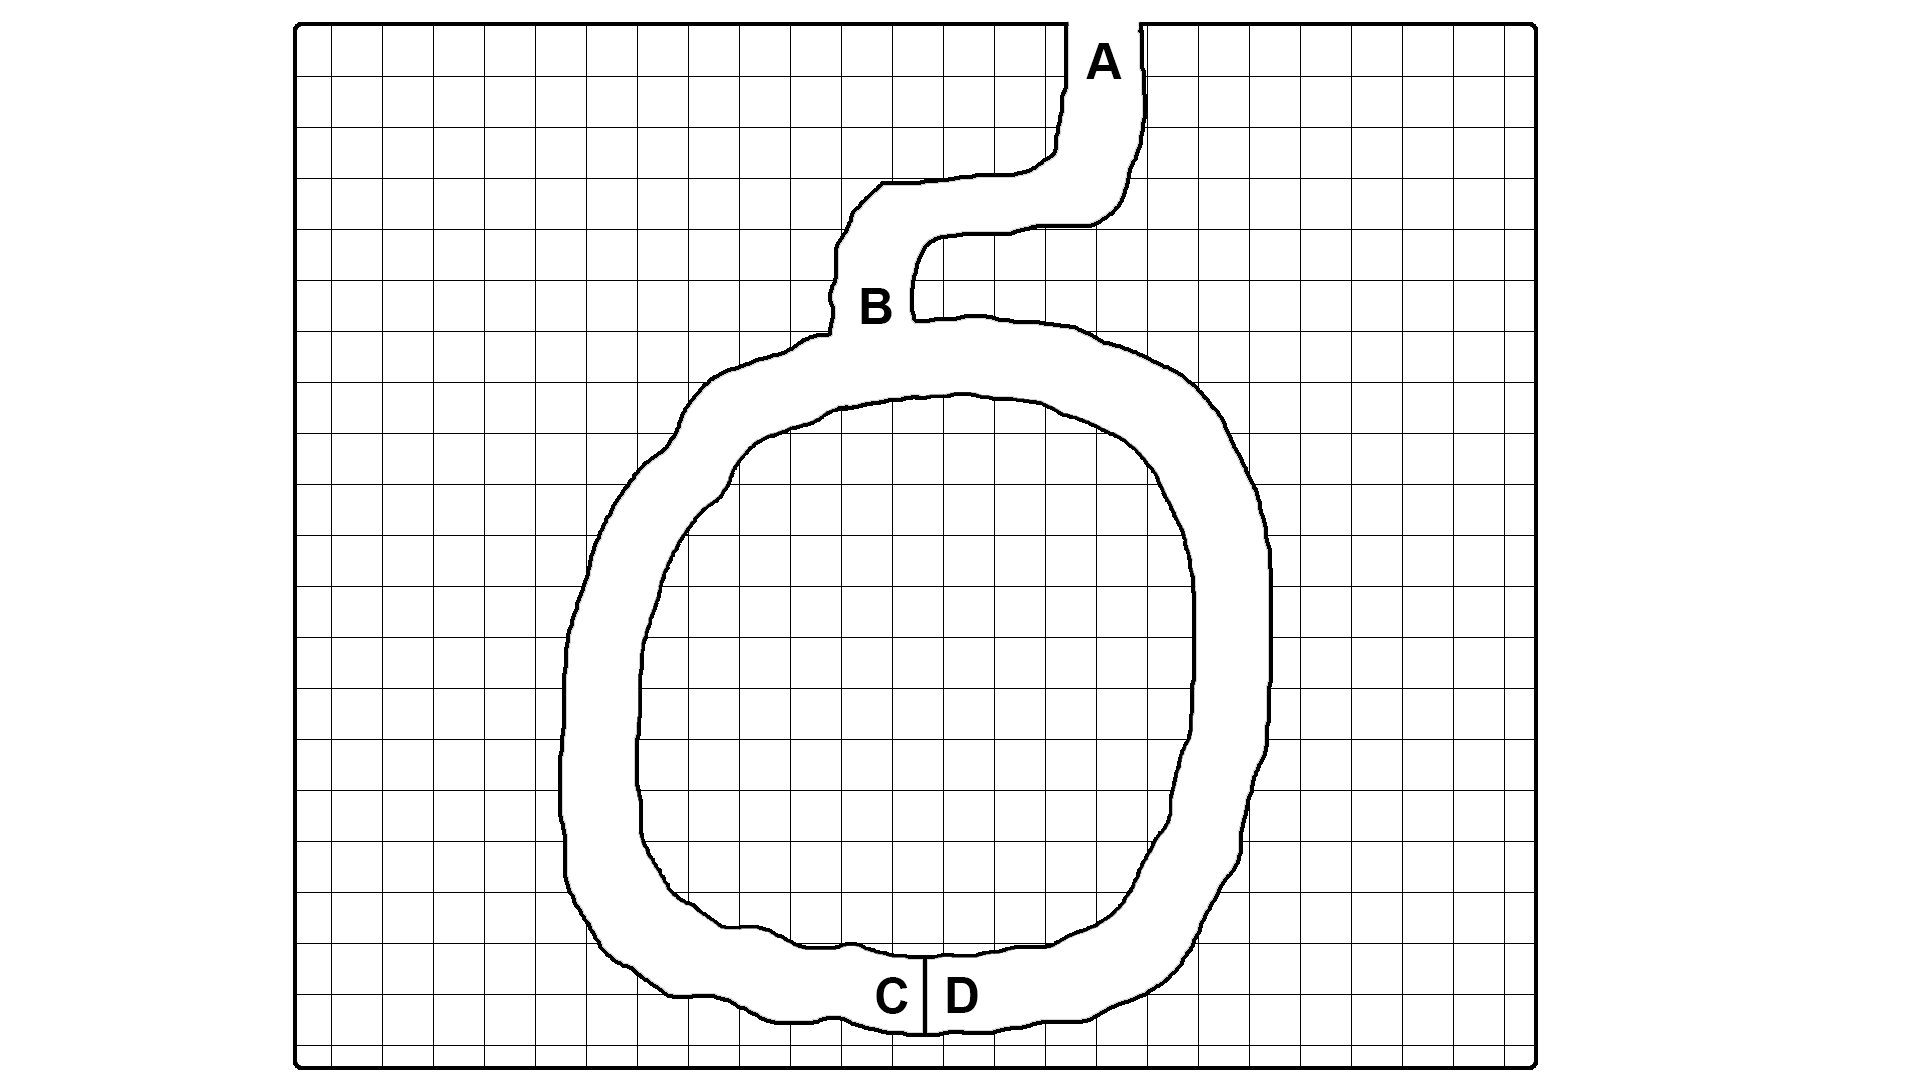
\includegraphics[width=0.6\textwidth]{ZKP.png}
    \caption{A nulla-ismeretű barlang.}
    \label{Figure::ZKcave}
\end{figure}

A többszöri ismétlésre azért van szükség, mert lehet Aladár be szeretné csapni Krisztát, amire minden iterációban 50\% esélye van. Ha abba az irányba ment amelyet Kriszta kiált, akkor szerencsésen be tudta őt csapni, azonban megfelelő ismétlésszámmal sokkal kevesebb esélye van Aladárnak.

A példa egy másik fontos jellemzője az, hogy Aladár ezzel bebizonyíthatta Krisztának, hogy tudja a jelszót, azonban Kriszta nem tud meggyőzni más arról, hogy Aladár tudja a jelszót. Tegyük fel, hogy Kriszta videót készített az egész folyamatról, de így se képes ő maga bizonyítani, hiszen mondhatjuk, hogy a felvétel hamisított, csalás.

Belátható, hogy ez egy nulla ismeretű protokoll, hiszen Kriszta számára bebizonyította Aladár, hogy ismeri a jelszót, méghozzá úgy hogy Kriszta semmit se tudott meg a jelszóról. Emellett Kriszta nem képes bizonyítani harmadik fél számára, hogy Aladár tudja a jelszót.

A nulla-ismeretű protokollokat Menezes, Oorschot és Vanstone a következő módon írták le formálisan könyvükben \citeyear{menezes1997handbook}:

Tekintsünk a nulla-ismeretű protokollokra kezdetben, mint interaktív bizonyítási rendszerekre (intaractive proof system), amiben a bizonyító és a hitelesítő felek többször is üzenetet váltanak. A bizonyjtó célja az, hogy valamilyen módon meggyőzze az hitelesítő felet, hogy birtokában van valamilyen tudásnak. A hitelesítő pedig elfogadhatja vagy elutasíthatja a bizonyítékot. A több üzenetváltásra azért van szükség, mert a bizonyíték egy interaktív játék formájában jön létre, ami egy inkább valószínűségi bizonyíték, mint abszolút bizonyíték. A hitelesítőn múlik, hogy milyen bizonyossággal rendelkező bizonyítékot fogad el, ez általában egy 1-hez rendkívül közeli érték szokott lenni.

Egy interaktív bizonyítékra azt mondjuk, hogy a \textit{tudás bizonyítéka} (proof of knowledge), ha rendelkezik a \textit{teljesség} (completeness) és \textit{megalapozottság} (soundness) tulajdonságokkal.

\begin{definition}
    \textbf{Teljesség.} Egy interaktív bizonyíték teljes, ha adott egy becsületes bizonyító és egy becsületes hitelesítő, valamint a protokoll sikeresen megy végbe (a hitelesítő elfogadja a bizonyító állítását).
\end{definition}

\begin{definition}
    \textbf{Megalapozottság.} Egy interaktív bizonyíték \textit{megalapozatlan}, ha létezik egy polinomiális algorimtus \textit{M} a következő tulajdonsággal: ha egy tisztességtelen bizonyító (megszemélyesíti Aladárt) nem elhanyogalható valószínűséggel sikeresen tudja végrehajtani a protokollt a hitelesítő féllel (Krisztával), akkor \textit{M} segítségével kinyerhető a a valódi bizonyító (Aladár) tudása/titka, amely így felhasználható a későbbiekben a protokoll futtatásakor.
\end{definition}

Mivel minden olyan félnek, aki képes Aladárt megszemélyesíteni, valójában a titokkal egyenértékű ismerettel kell rendelkeznie, a \textit{megalapozottság} tulajdonság garantálja, hogy a protokoll valóban előállítja a \textit{tudás bizonyítékát}. Így ez a tulajdonság megakadályozza a csalókat.

Míg a fenti tulajdonságok lefekteti a nulla-ismeretű protokollok alapját, a legfőbb tulajdonság, amiről a nevüket is kapták, a \textit{nulla-ismeret}.

Azonban mielőtt kitérnénk erre a definícióra, szükséges megismernünk mik is a \textit{szimulátorok}. A barlangos példa esetében előjött egy eset, hogy Kriszta felvételt készít Aladár bizonyításáról és beláttuk hiába mutatja azt meg egy harmadik félnek, ő nem fogja elhinni, mert nem megbízható a felvétel mint bizonyíték (könnyen hamisítható). A harmadik fél csak úgy lenne meggyőzhető, ha Aladár eljátszaná a bizonyítást a harmadik fél által választott szekvenciára. Ha létezik olyan módszer, amellyel készíthető az eredetitől megkülönböztethetetlen bizonyíték, akkor azt mondjuk hogy létezik \textit{szimulátor} a bizonyítékra.

\begin{definition}
    \textbf{Nulla-ismeret.} Egy \textit{tudás bizonyítéka} protokoll, rendelkezik a nulla-ismeret tulajdonsággal, ha szimuláltható a következő módon: létezik egy polinomiális algoritmus (\textit{szimulátor}), amely a valódi bizonyító féllel való együttműködés nélkül képes az bemenetnek megfelelő átiratot készíteni, amely megkülönböztethetetlen a valódi bizonyító féltől kapottól.
\end{definition}

A \textit{nulla-ismeret}-ből következik, hogy ha a bizonyító fél végrehajtja a protokollt, azzal nem ad ki semmilyen információt a titokról, csupán bizonyítja a tudását. Így akárhányszor is bizonyítja, a megszemélyesítése nem lesz egyszerűbb.
    \chapter{Nulla-ismeretű protokollok azonosításra}

A nulla-ismeretű protokollok egyik elterjedt alkalmazása a felhasználók azonosítása, autentikálása. Ebben a fejezetben ilyen protokollokat fogunk áttekinteni.

\section*{A Schnorr azonosító protokoll}

Ezt megelőzően is léteztek már nulla-ismeretű protokollok, mint Fiat-Shamir \cite{FiatShamir} és annak továbbfejlesztései (FFS \cite{FeigeFiatShamir} és GQ protokollok \cite{GuillouQuisquater}), amelyek biztonsságosságukat a faktorizációs probléma nehézségéből nyerik. 

A Schnorr protokoll \cite{Schnorr}, ezzel ellentétben biztonságát a diszkrét logaritmus problémából nyeri. Manapság az elliptikus görbe kriptográfia egyre nagyobb teret nyer, köszönhetően a kisebb kulcsméretnek, vele együtt pedig növekszik az elliptikus görbe diszkrét logaritmus probléma. Ezért úgy érzem előnyösebb Schnorr protokollját áttekinteni, mint az őt megelőző faktorizáción alapuló protokollokat.

\subsection*{A diszkrét logaritmus probléma}\cite{BerczesPetho}

\begin{definition}
    Legyen $m$ egy pozitív egész szám. Egy $g$ egész számot primitív gyöknek nevezünk modulo $m$ ha minden $b \in \{1,2,...,m-1\}$ szám esetén, melyre $(b,m) = 1$ létezik olyan $k$ pozitív egész szám, melyre $g^k \equiv b \pmod{m}$.
\end{definition}

\begin{theorem}
    Akkor, és csakis akkor létezik primitív gyök modulo $m$, ha $m = 2$, $m = 4$, $m = p^k$ vagy $m = 2p^k$, ahol $p$ valamely pozitív szám.
\end{theorem}

\begin{definition}
    Legyen $p$ egy pozitív prímszám, $b$ egy egész szám, melyre $(b, p) = 1$, és legyen $g$ egy primitív gyök modulo $p$. Azt a legkisebb pozitív egész $k$ számot, melyre teljesül, hogy $g^k \equiv b \pmod{p})$ a $b$ szám $g$ alapú diszkrét logaritmusának nevezzük modulo $p$.
\end{definition}

Miközben a modulo $p$ történő hatványozás nagy $p$ értékek esetén is gyorsan kiszámítható, addig ennek megfordítása, a diszkrét logaritmus kiszámítása nagyon időigényes feladat.

\subsection*{A Schnorr azonosító protokoll algoritmusa}

A protokol a rendszer paraméterek inicializáló lépésével indul.

\begin{algorithm}[H]
    \floatname{algorithm}{Algoritmus}
    \caption{Rendszer inicializáció}
    \label{algorithm:systemInit}
    \begin{algorithmic}
        \Procedure{sys\_init}{$t$} \Comment $2^{-t}$ a rendszerben a helyes tippelés valószínűsége
        \State $p$ prím inicializálása
        \State $q$ prím inicializálása \Comment $q | p-1$
        \State $\alpha$ elem kiválasztása \Comment $\alpha \in \mathbb{Z}_{p}$ és rendje $q$
        \EndProcedure
    \end{algorithmic}
\end{algorithm}

\begin{algorithm}[H]
    \floatname{algorithm}{Algoritmus}
    \caption{Felhasználói paraméterek generálása}
    \label{algorithm:userInit}
    \begin{algorithmic}
        \Procedure{user\_init}{$I_{A}$} \Comment $I_{A}$ a felhasználó egyedi azonosítója
        \State $s$ privát kulcs generálása \Comment ez egy random szám az $\{1,2,...,q\}$ halmazból
        \State $v = \alpha^{-s} \pmod{p}$ publikus kulcs kiszámítása
        \State $\alpha$ elem kiválasztása \Comment $\alpha \in \mathbb{Z}_{p}$ és rendje $q$
        \State A rendszerrel aláíratja az $(I_{A}, v)$ párost, ezzel előáll $sign_{A}$
        \EndProcedure
    \end{algorithmic}
\end{algorithm}

Ezt követően az azonosító protokoll-t mutatja a \ref{Figure::SchnorrProt} ábra:

\begin{figure}[H]
    \centering
    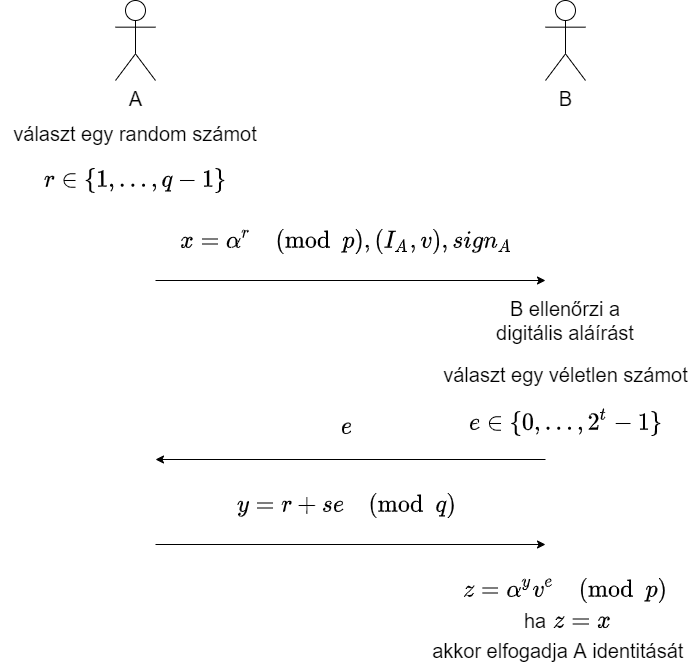
\includegraphics[width=0.6\textwidth]{Schnorr-protokoll.png}
    \caption{Schnorr azonosító protokoll.}
    \label{Figure::SchnorrProt}
\end{figure}

\subsection*{A Schnorr azonosító protokoll biztonságossága}

\begin{itemize}
    \item Biztonság: A biztonságosság egyik fő szereplője a $t$, ezt olyan módon kell megválasztani, hogy $2^{-t}$ kellően kicsi legyen, hiszen ez a valószínűsége a helyes tippelésnek a választott $e$ értékre. A másik fontos pontja a protokollnak a megfelelő méretű $q$ választása, mert ez felelős a diszkrét logaritmus probléma nehézségéért.
    \item Megalapozottság: A protokollt áttekintve, belátható, hogy $s$ ismerete nélkül nem lehetséges senki számára, hogy $A$-nak adja ki magát, mert ezen információ ismeretében képes csak sikeresen végigjátszani a folyamatot.
    \item Nulla-ismeret: A protokoll csak akkor teljesíti a nulla-ismeret tulajdonságot, ha a hitelesítő fél becsületesen jár el. Ez azt jelenti, hogy az $e$ értéket valóban random módon választja ki és nem a kapott $x$ értékétől függően. Ha $x$ értéke alapján választ egy számára megfelelő $e$-t, akkor képes információt kinyerni a felhasználó a bizonyító fél titkával kapcsolatban.
\end{itemize}

\begin{minipage}{\textwidth}
Ezen felül rendkívül fontos követelménye ennek a protokollnak, hogy egy interaktív folyamat során ne használjuk kétszer ugyanazt a random $r$ értéket, hiszen ha kétszer használnánk egyszerűen kiszámíthatóvá vális az $s$ titkunk a következő módon:

$(y_1 - y_2) / (e_1 - e_2) \pmod{q}$ \\
$= (r + se_1) - (r + se_2) / (e_1 - e_2) \pmod{q}$ \\
$= s(e_1 - e_2) / (e_1 - e_2) \pmod{q}$ \\
$= s$
\end{minipage}

\section*{M-Pin protokoll}

Az M-Pin protokoll \cite{MPin} egy rendkívül modern elgondolása az autentikációnak, ami a jelenlegi felhasználónév és jelszó alapú rendszerek egy működőképes alternatívája. Ahogy korábban is említettem a jelszavas rendszerek nagy hátránya, hogy a szervereken létezik egy adatbázis amiben a felhasználói jelszavak tárolásra kerülnek többnyire hash-elt változatban (azonban még előfordulnak olyan esetek is, amikor a tényleges jelszót tárolják). Ezeket az adatbázisokat gyakran feltörik és ellopják.

Az M-Pin célja az, hogy a regisztrált felhasználóknak osszunk ki egy nagy kriptográfiai titkot, amelyet felhasználva nulla-ismeretű bizonyítékkal képes igazolni kilétét. Így nincs szükség arra, hogy bármilyen felhasználói titkot tároljon a szolgáltató a szerverein.

Mielőtt áttekintenénk, hogyan is működik ez az eljárás, fontos ismernünk az elliptikus görbék és a párosítás alapjait.

\subsection*{Elliptikus görbe kriptográfia}

A témáról kimerítően a \cite{ECCGuide, ECCHandbook} könyvekben lehet olvasni, én csupán a protokoll megértéséhez szükséges részleteket szeretném áttekinteni.

A kriptográfiában kiemelt szereppel bírnak az úgynevezett Weierstrass elliptikus görbék: $$y^2 = x^3 + ax + b.$$ Egy ilyen görbéről látható példa a \dotref{Figure::ECC::EllipticCurve} ábrán.

\begin{figure}[H]
    \centering
    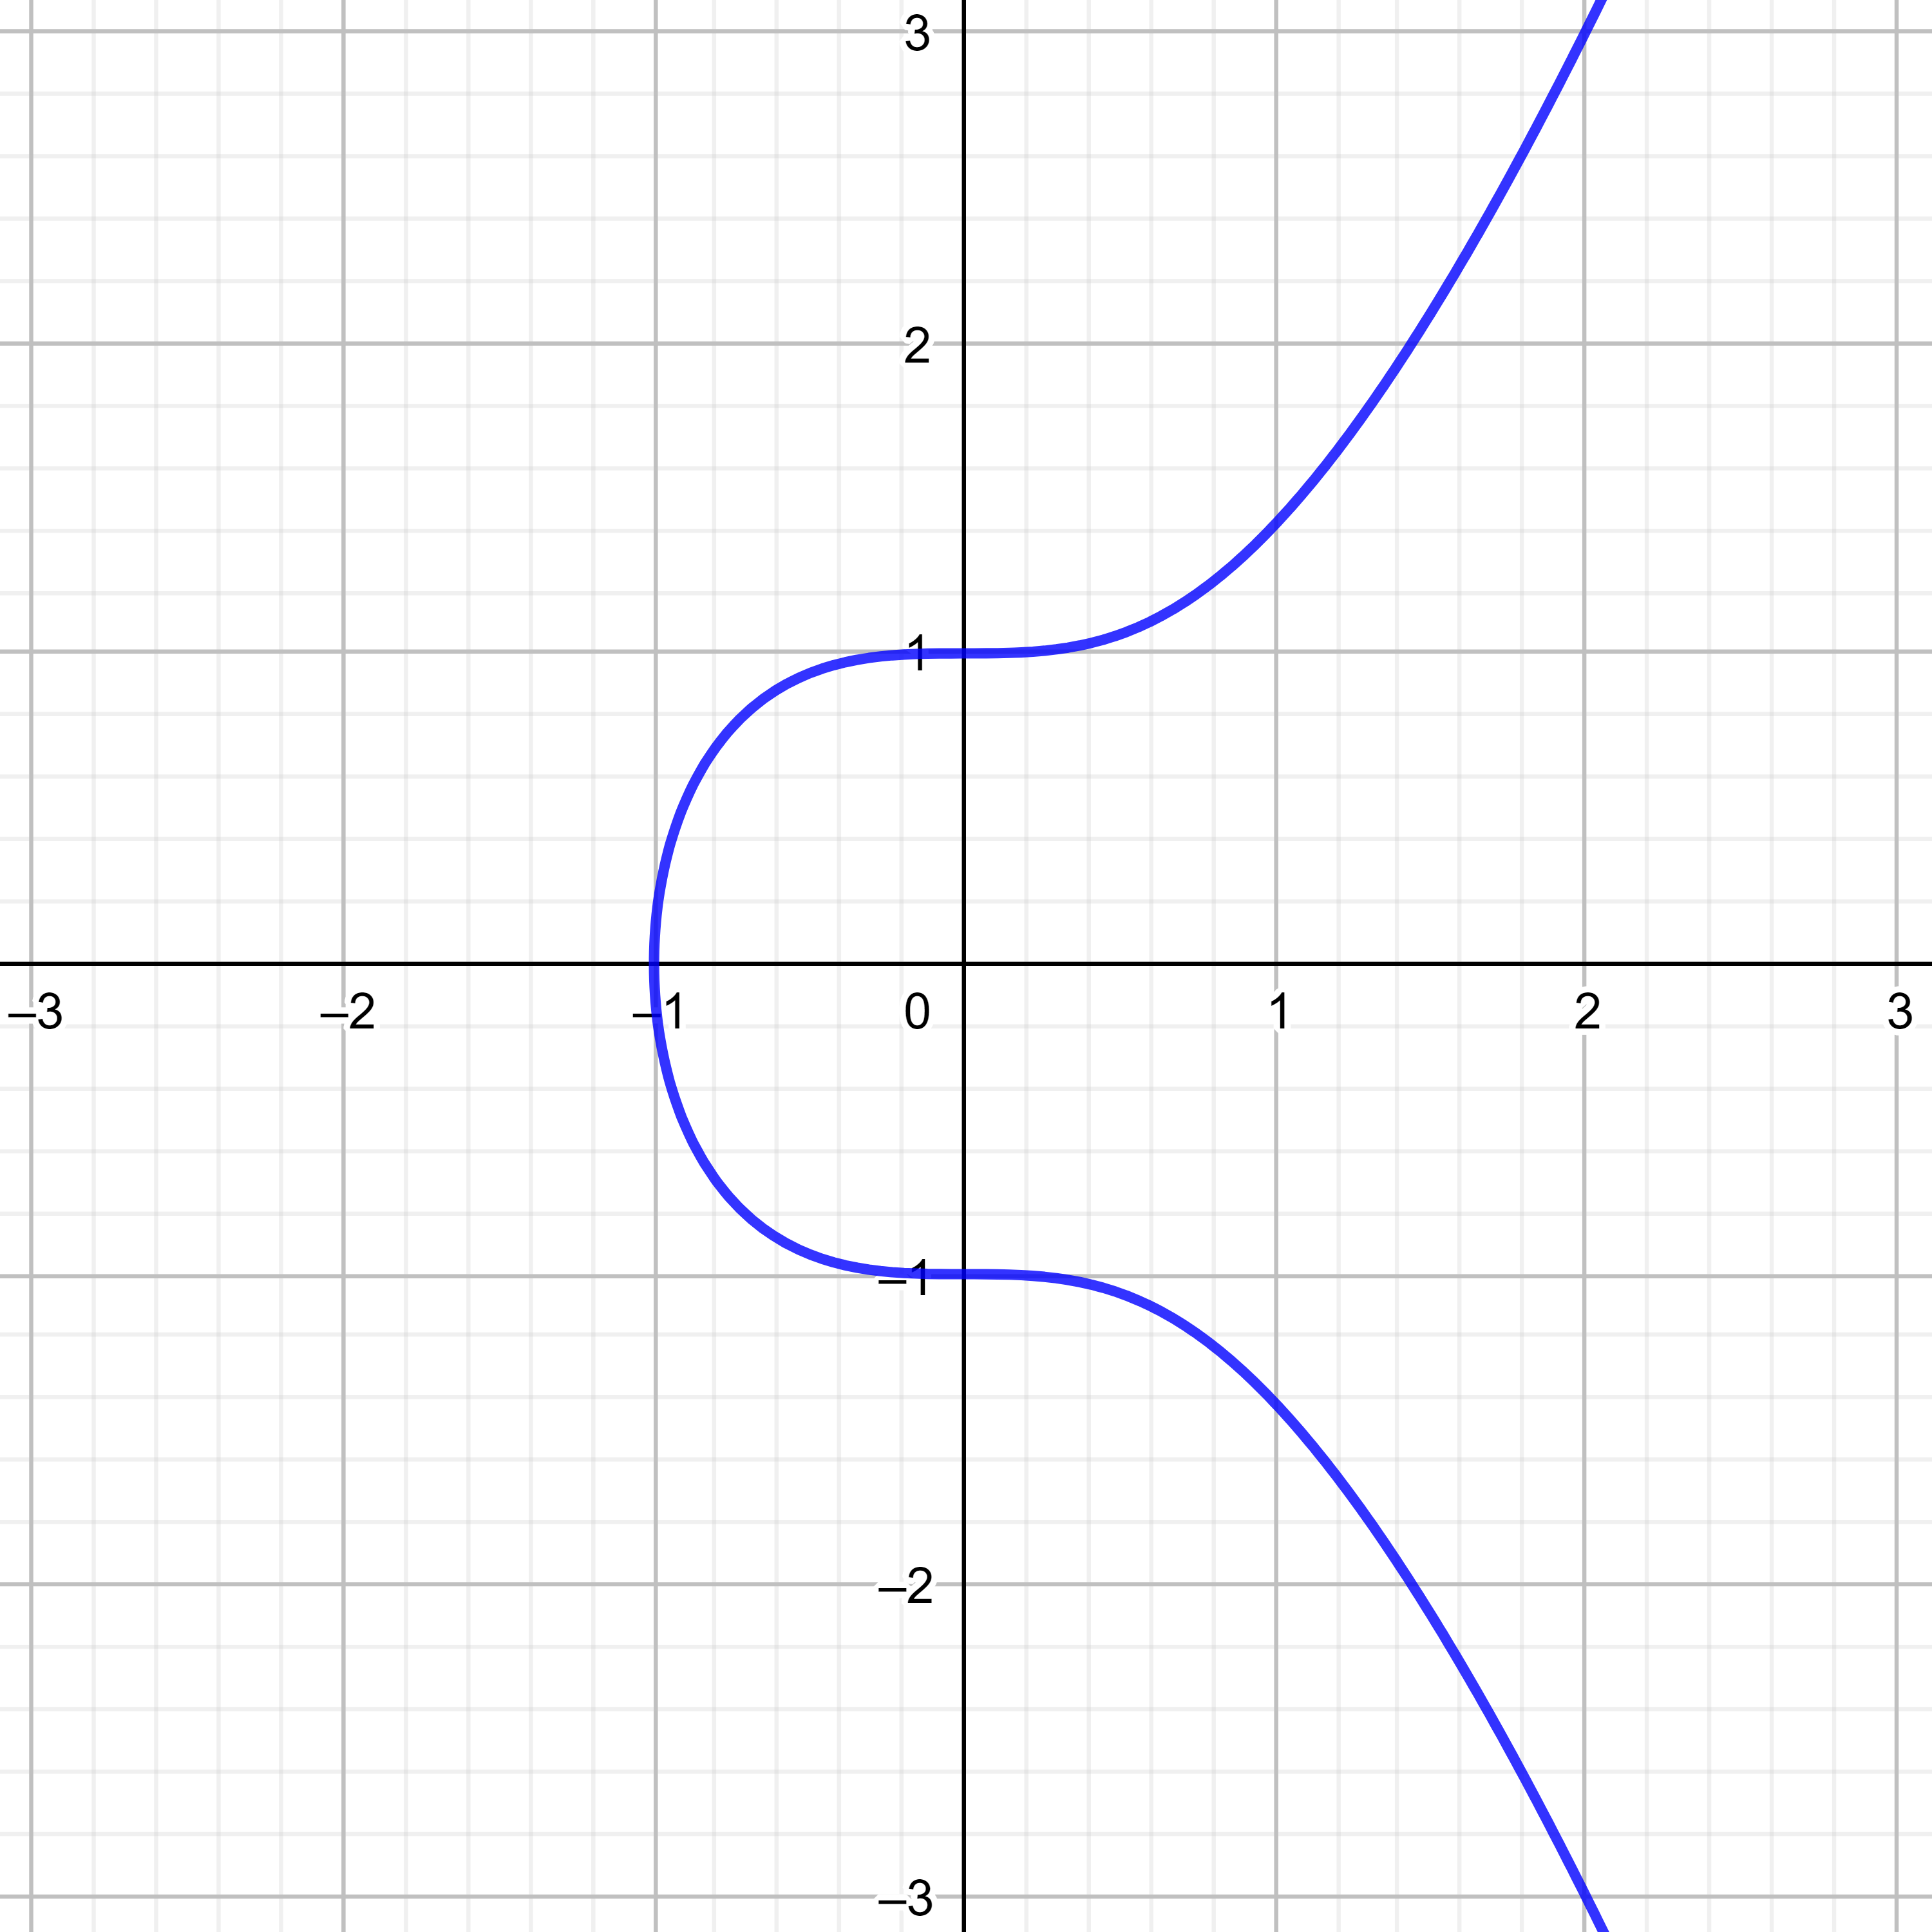
\includegraphics[width=0.4\textwidth]{elliptikus-gorbe.png}
    \caption{Az $y^2 = x^3 + 1$ görbe a valós számok teste felett.}
    \label{Figure::ECC::EllipticCurve}
\end{figure}

\subsubsection*{Az $E(K) : y^2 = x^3 + ax + b$ görbe tulajdonságai \protect\footnote{Ha $K$ karakterisztikája nem $2$.}}

\begin{outdentlist}
    \item[]
    \textbf{Egységelem.} $P + O = O + P = P$, minden $P \in E(K)$ esetén.

    \item[]
    \textbf{Ellentettek.} Ha $P = (x, y) \in E(K)$, akkor $(x, y) + (x, -y) = O$. Az $(x, -y)$ pontot $-P$-vel jelöljük és $P$ ellentettjének nevezzük. $-P$ is $E(K)$ egy pontja.

    \item[]
    \textbf{Pontok összeadása.} Legyen $P = (x_1, y_1) \in E(K)$ és $Q = (x_2, y_2) \in E(K)$, úgy hogy $P \neq \pm Q$. Ekkor $P + Q = (x_3, y_3)$, ahol 
    \begin{center}$x_3 = \big(\frac{y_2 - y_1}{x_2 - x_1}\big)^2 - x_1 - x_2$ és $y_3 = \frac{y_2 - y_1}{x_2 - x_1}(x_1 - x_3) - y_1$.\end{center}

    \item[]
    \textbf{Pont duplázás.} Legyen $P = (x_1, y_1) \in E(K)$, úgy hogy $P \neq -P$. Ekkor $2P = (x_3, y_3)$, ahol
    \begin{center}$x_3 = \big(\frac{3x_1^2 + a}{2y_1}\big)^2 - 2x_1$ és $y_3 = \frac{3x_1^2 + a}{2y_1}(x_1 - x_3) - y_1$.\end{center} Ha $P = -P$, akkor $2P = O$.

    \item[]
    \textbf{Pontok skalár szorzása.} Legyen $P \in E(K)$ és $n \in \mathbb{Z}$. Ekkor egy lehetséges módszer a skalár szorzásra a \textit{Double-and-Add} módszer: $$nP = \sum_{i = 0}^{t-1} n_i 2^i(P) = n_0P + 2(n_1P + 2(n_2P + 2(... + 2(n_{t-1}P)...))).$$
\end{outdentlist}

Most, hogy ismerjük a műveleteket, bemutatom a protokoll szempontjából fontos tulajdonságot a disztibutivitást az elliptikus görbéken.

Legyenek $n \in \mathbb{Z}$ és $P \in E(K)$, ha $n = n_1 + n_2$, akkor $nP = n_1P + n_2P$. Továbbá, legyen $P_1, P_2 \in E(K)$, ekkor $n(P_1 + P_2) = nP_1 + nP_2$.

Azonban az elliptikus görbe kriptográfia legfontosabb tényezője az elliptikus diszkrét logaritmus probléma, ami egy nehezen megoldható probléma.

\begin{definition*}
    Az \textbf{elliptikus diszkrét logaritmus probléma} (ECDLP): Adott egy $E$ elliptikus görbe az $\mathbb{F}_q$ véges test felett, egy $n$ rendű $P \in E(\mathbb{F}_q)$ pont, valamint egy $Q$ pont, amely $P$ többszöröse. Keressük azt az $l \in [0, n - 1]$ egész számot, amelyre $Q = lP$ teljesül. Ezt a számot a $Q$ pont $P$ alapú elliptikus diszkrét logaritmusának nevezzük.
\end{definition*}

\subsection*{Párosítás-alapú kriptográfia}

A párosításról és a kriptográfiában való alkalmazásáról részletes olvasmány a Guide to pairing-based cryptography \cite{PBCGuide}. Számunkra azonban elegendő a párosítás műveletének tulajdonságait ismerni, továbbá azt, hogy a párosítás alkalmazásával komplex matematikai problémákat vagyunk képesek redukálni azzal, hogy egy másik csoportba visszük át a problémát.

Jelöljön $G_1, G_2$ additív, míg $G_\mathbb{T}$ multiplikatív $r$ rendű csoportokat. Az $e$ párosítás egy olyan $e : G_1 \times G_2 \rightarrow G_\mathbb{T}$ leképezés, amely a következő tulajdonágokkal rendelkezik:
\begin{outdentlist}
    \item[] \textbf{Bilineáris.} Jelölje $\mathbb{Z}_r$ az egész számok halmazát modulo $r$, ekkor $\forall P_1 \in G_1, P_2 \in G_2$ és $a, b \in \mathbb{Z}_r$ esetén $e(aP_1, bP_2) = e(P_1, P_2)^{ab}$.

    \item[] \textbf{Nem elfajuló.} Ha $P_1 \neq 0_{G_1}$ és $P_2 \neq 0_{G_2}$, akkor $e(P_1, P_2) \neq 1_{G_\mathbb{T}}$, ahol $0_{G_1}$ (illetve $0_{G_2}$ és $1_{G_\mathbb{T}}$) az egységeleme a $G_1$ csoportnak (illetve $G_2$ és $G_\mathbb{T}$ csoportnak).

    \item[] \textbf{Hatékonyan számítható.}

    \item[] \textbf{Nehezen megfordítható.}
\end{outdentlist}

\subsection*{Az M-Pin protokoll algoritmusa}
    \chapter{Tobábbi nulla-ismeretű protokollok}

Ezen fejezet célja, hogy az azonosításon túl további felhasználási lehetőségeit mutassam be a nulla-ismeretű protokolloknak. Tényleges protokollokat nem fogunk tekinteni, csupán ötleteket és azok előnyeit.

Mielőtt a következő protokollokat tárgyalnánk, szükséges megismerkednünk a \textit{proof of knowledge} mellett az \textit{argument of knowledge} definícióval, ami annyiban különbözük, hogy a \textit{megalapozottság} tulajdonság esetén a statisztikai követelményt számítási követelménnyé gyengíti. Tehát, míg előbbi esetben a bizonyító fél korlátlan számítási kapacitással bír, addig utóbbiban polinomiálisan kötött számítási kapacitással számolunk.

\section{Nem-interaktív nulla-ismeretű protokollok}

A nulla-ismeretű protokollok közül eddig csupán interaktív protokollokról volt szó, azonban rendkívül elterjedt az interaktivitást nem követelő protokollok alkalmazása is. Ezen protokollok megszületését az a probléma indokolta, hogy az interaktivitás számos oda-vissza történő kommunikációt igényel és míg a számítások gyorsan elvégezhetők, az esetenként akár több száz adatcsere közel sem elhanyagolható kölcségekkel jár. 

Az ilyen protokollok \cite{NIZK, NIZK2} alapötlete, hogy létezzen valamilyen mindenkinek elérhető formában olyan random adat, amely rendelkezik a "well mixedness" tulajdonsággal, ami nem egy kézzel fogható tulajdonság, definíciót a szerzők se adtak. Felfoghatjuk úgy, hogy kriptográfiailag biztonságos random generátorral készült adat.

Ezzel a módszerrel a kommunikáció egyirányúvá válik, hiszen a hitelesítő fél feladata, hogy random értéket küldjön a bizonyító félnek helyettesítésre került a publikus random adattal, így minimális módosítással csökkenthettük protokollunk komplexitását, méghozzá úgy, hogy a nulla-ismeretű protokollok alaptulajdonságai nem sérülnek.

\section{Succinct non-interactive arguments of knowledge - SNARK}

Az interaktivitás elhagyásával sikerült kisebb komplexitással rendelkező protokollokat készíteni és ezt felhasználva a gyakorlatban is alkalmazni őket. Továbbra is probléma volt azonban, hogy sok esetben a bizonyító fél által küldött üzenet mérete nagy volt. Például, ha kis számítási kapacitással rendelkezünk és a számítást kiszervezzük valamilyen felhőszolgáltatónak, azonban szeretnénk valamilyen bizonyítékot is kapni a számítás helyességéről, akkor olyan protokoll alkalmazása szükséges használni, amely a kis számítási kapacitással bíró felhasználót nem terheli meg. Erre kompakt és számításigényét tekintve könnyű argumentumok alkalmazása szükséges. Ilyen protokollok például a SNARG (succinct non-interactive argument), vagy a SNARK (succinct non-interactive argument
of knowledge).

Egy kurrens protokoll a \cite{SNARK}, amelyet blockchain alapú kriptovaluták esetén előszeretettel alkalmaznak (Zcash\footnote{https://z.cash/technology/zksnarks/}, Filecoin\footnote{https://filecoin.io/}). Számos nyílt forráskódú megvalósítása létezik: \href{https://github.com/scipr-lab/libsnark}{libsnark}, \href{https://github.com/zkcrypto/bellman}{bellman}, \href{https://github.com/scipr-lab/dizk}{dizk}, \href{https://github.com/iden3/wasmsnark}{wasmsnark}.

STARKs \cite{STARK}

Bulletproofs \cite{BULLETPROOF}

    \bibliography{references}
\end{document}
